\section{Introduction}
\textbf{The purpose of this section is to elaborate a bit on the abstract and to provide a clear picture of the structure for this thesis. Starting with speculations on the nature of dark matter based on current observational constraints we can set up the appropriate theoretical framework and introduce some important concepts to describe collisionless systems. This chapter ends with the general notion of an attractor and some ideas for where to search for it in terms of dark matter systems (if it exists).} \\ \\

Advancements has been made in narrowing down the window of theoretically allowed DM particles through modern observational constraints (upper bounds to DM cross sections are lowered further as more and more DM structures aids in the vast collection of constraining structures, e.g. the bullet cluster where gravitational lensing of background objects shows two huge parts of hidden mass as remnants of the merger between two galaxy clusters with their individual dark halos (the hot X-ray gas remains in the center as it is subjected to numerous collisions intrinsically). Most astronomers believe dark matter candidates to be in the form of one or several new types of elementary particles (existing outside the current standard model of particle physics).

\centerline{\textbf{Theoretical framework}} 

\centerline{\textbf{Quantum effects are negligible}} 
Utilizing Ehrenfests theorem since the mean inter-particle distance in each simulation in the present work is larger than the particles Debroglie wavelength $\lambda = \frac{h}{p}$, we can neglect any quantum mechanical treatment and rely solely on a classical mechanical treatment for our purpose here. 
It is not known if particle collisions are important in real halos. 
Probably this will not play a role in Milky way-like galaxies but in dwarf galaxies it might [12].

\centerline{\textbf{The Newtonian limit is applicable}} 
General Relativity (GR) can also be safely neglected here, as all three conditions for taking the Newtonian limit is met ($v<<c$, $\frac{GM}{R}<<1$ in dimensionless units, and finally the structures in this work posses almost static gravitational potentials where the time-dependence is negligible). Newtonian Dynamics is therefore the appropriate theoretical framework to use (see [13] and [14]). \\

As a consequence to the fact that DM structures have a smooth density field, seem to be collisionless, and must be cold (individual particle velocities much less than the speed of light in vacuum, $v << c $. Plus we know that galaxies form befor e the formation of clusters which severely constrains the allowed ratio of hot to cold matter.), the MACHOs (MAssive Compact Halo Objects) have more or less been ruled out and WIMPS (Weakly Interacting Massive Particles) remain a top category candidate for the nature of DM. Other candidates of interest are SUper SYmmetric (SUSY) particles, axions etc. Modifications to our current understanding of gravity such as MOND or TeVeS are also considered by some. Furthermore, as any DM particle candidates obeying the above criteria (e.g. fitting in the remaining allowed energy range with a mass that is not too large) must be very numerous to account for the total density parameter value of DM (with best modern estimates, $\Omega \approx 0.23$). It is therefore necessary to have an effective measure to qualitatively describe the physical quantities of interest for the DM structures that does not depend on a detailed description of orbit etc. for each individual particle but instead treats the structures in a probabilistic manner. For this purpose the Distribution Function (DF) is introduced. The DF $f(x,v,t)$ has the three arguments of position, velocity and time. At any given time it therefore describes collective phenomena in a 6D-phasespace. The probability of finding a given particle at time t in the 6D-phasespace volume $d^3xd^3v$ is given by $f(x,v,t)d^3xd^3v$. (This gives the particle mass inside that 6D volume when multiplied by the total mass). Assuming the DM particles are belonging to just one species,i.e. they are indistinguishable, that probability is unchanged for each of the N particles inside any given DM structure. This assumption implicates a normalization for the DF at unity:
\begin{equation}
\int \! f(x,v,t) \, \mathrm{d^3}x \mathrm{d^3}v = 1
\end{equation}
Taking the Continuity Equation (CE) into account and translating it into a conservation of probability,
\begin{equation}
\frac{\partial f}{\partial t} + \frac{\partial}{\partial w}\cdot (f\dot{w}) = 0
\end{equation}
where $w = (r,v)$ and $ \dot{w} = (\dot{r},\dot{v}) = (v, a ) = (v, -\nabla \Phi ) $, where a is the acceleration and $\nabla \Phi$ is the gradient of the gravitational potential. This conservation in phase space of probability basically means, that when we follow a certain particles trajectory, the probability of finding it within a surrounding, co-moving phase space element stays the same. With the use of Hamiltons equations, the Collisionless Boltzmann Equation (CBE) can be obtained (See appendix D.4). Here written for simplicity in the form of the convective/Lagrangian derivative of the DF: \\
\begin{equation}
\frac{df(x,v,t)}{dt} = 0 
\end{equation}
Taking the 1.st moment of the CBE (Multiplying each term in the CBE by the radial momentum, and subsequently integrating over all momenta) gives us a very useful expression, namely the Jeans Equation (JE) (see derivation in appendix D.5). With no bulk motion, and assuming spherical symmetry as well as dynamical equilibrium the JE reads:
\begin{equation}
v_c^2 = -\sigma_r^2  \big[\gamma +\kappa +2 \beta \big] 
\end{equation}
with the circular velocity,
\begin{equation}
v_c^2 = \frac{GM}{r}
\end{equation}
There is evidence pointing to the fact that dark matter might be collisionless described by the velocity anisotropy parameter, 
\begin{equation}
\beta \equiv 1 - \frac{\sigma_{tan}^2}{2 \sigma_{rad}^2} 
\end{equation}
where $\sigma_{tan}$ and $\sigma_{rad}$ are the tangential and radial velocity dispersions, respectively. It is known from cosmological simulations that $\beta$ increase from zero at the center of a halo to about $\beta \approx 0.25$ at $r_{-2}$, which is the radius where $\gamma = -2$, with the radial slope of the density profile , 
\begin{equation}
\gamma \equiv \frac{d\ln\rho}{d\ln r}
\end{equation}
finally the radial slope of the radial velocity dispersion is defined as
\begin{equation}
\kappa = \frac{d\ln\sigma_r^2}{d\ln r} 
\end{equation}
The JE thus closely resembles the formula for Hydrostatic Equilibrium (HE), which becomes more clear if $\sigma_r^2$ is interpreted as temperature and $\kappa$ thus becomes the radial part of the temperature gradient. 

\begin{figure}[!htbp]
\centering
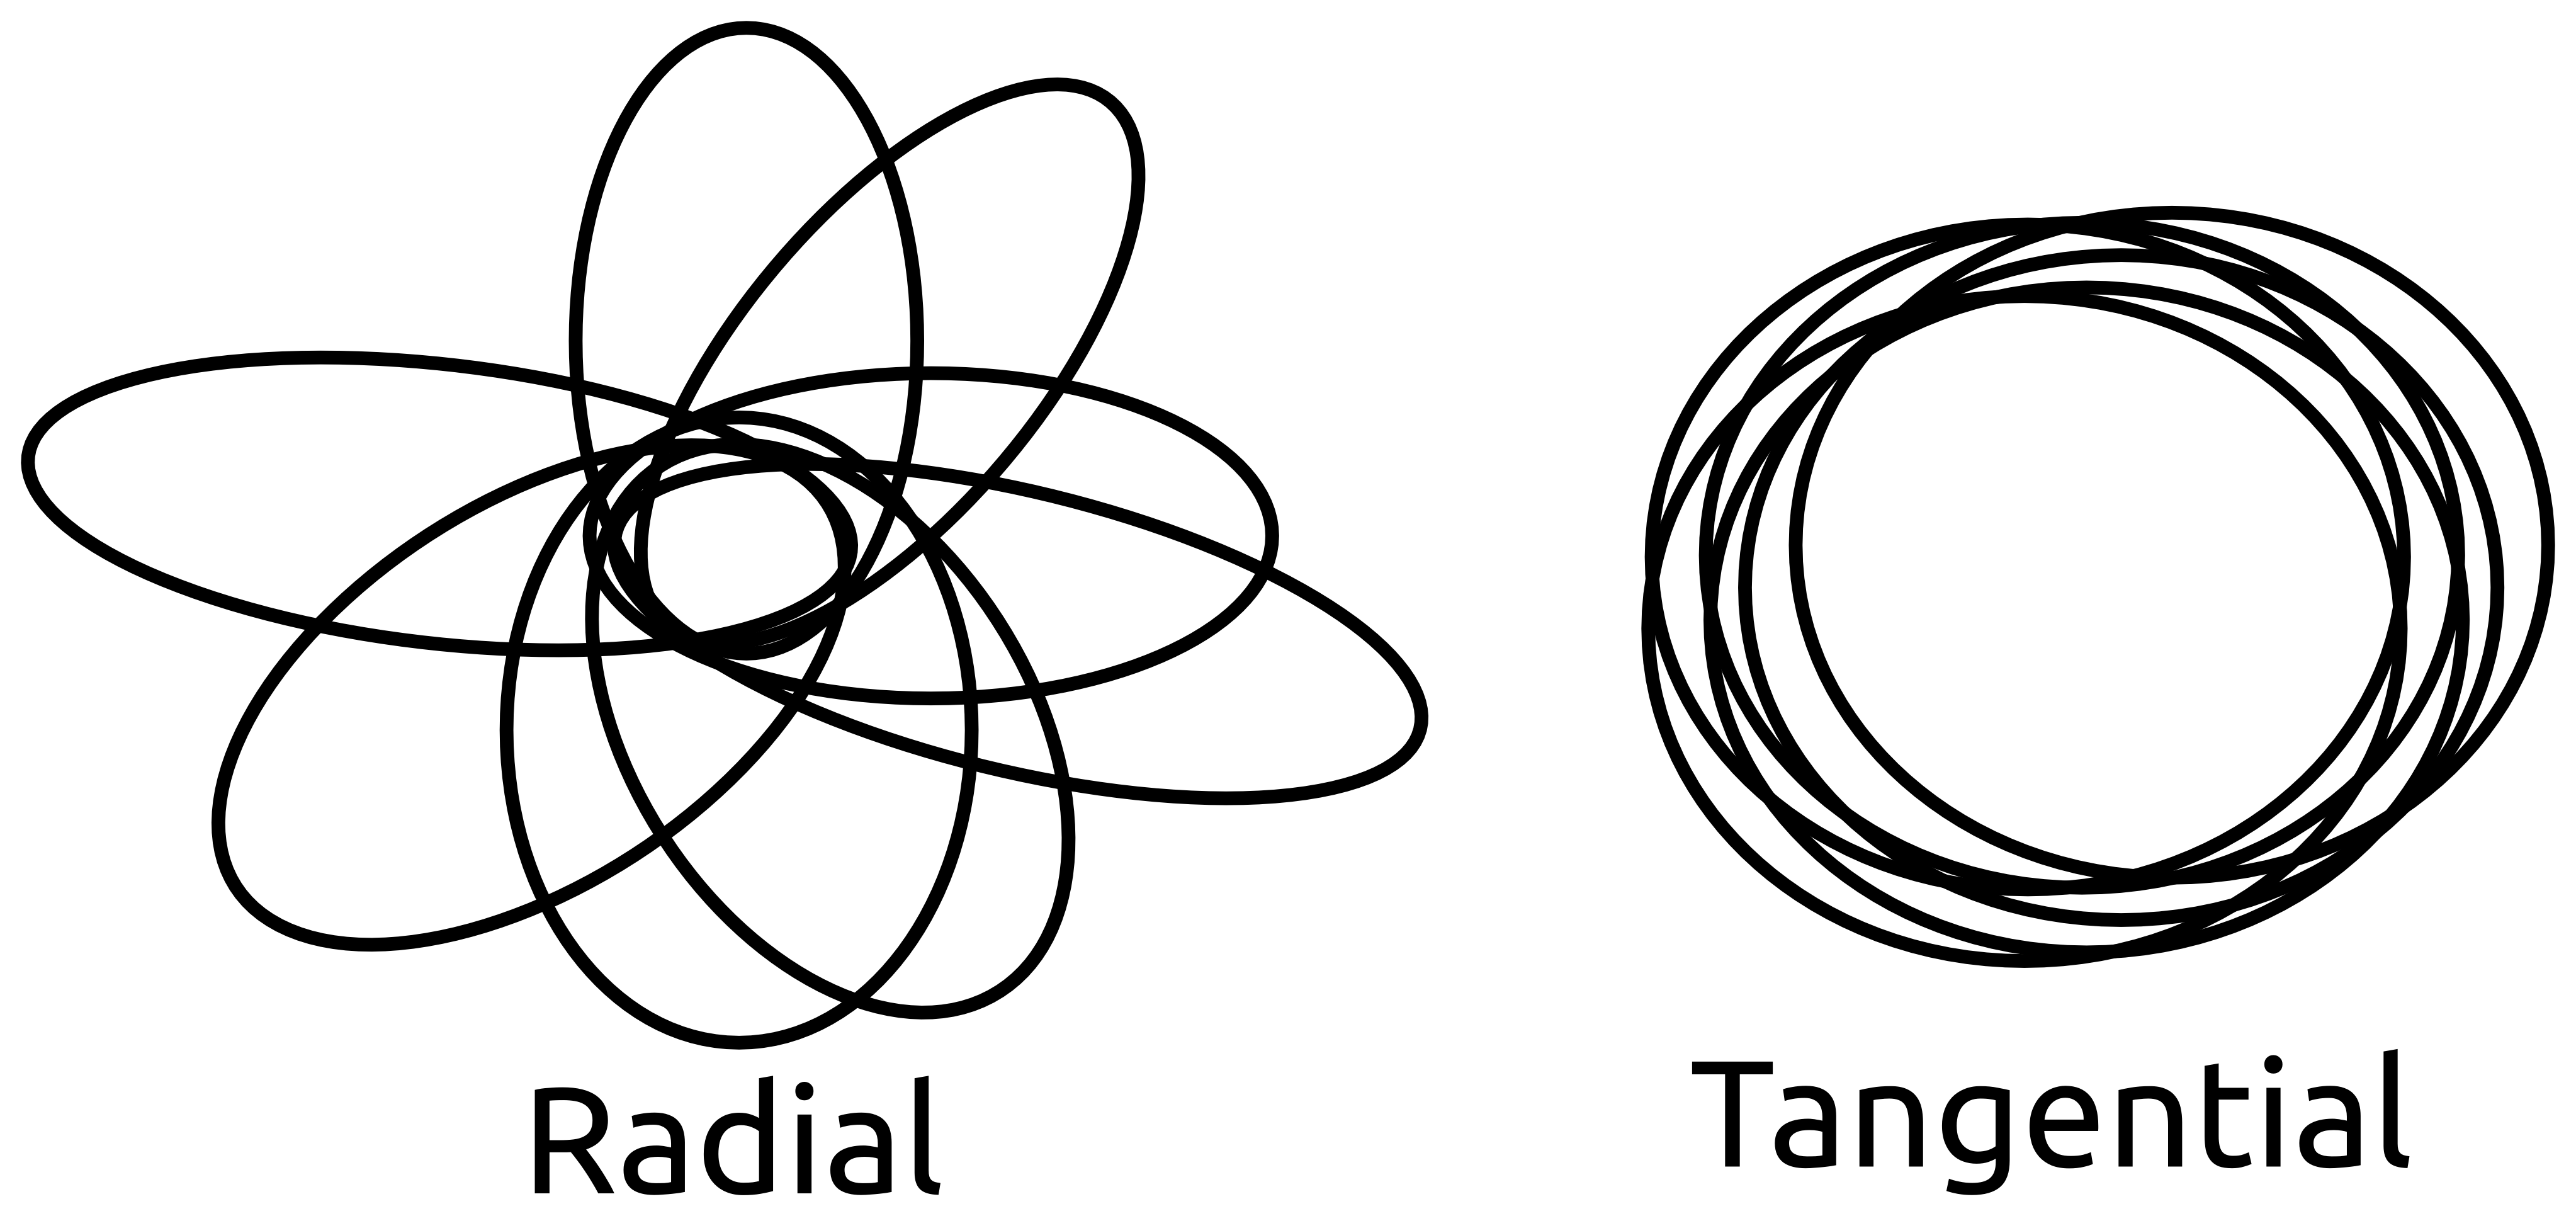
\includegraphics[width=1.0\linewidth]{Thesis_Final_Version/img/orbit.png}
\caption{Radially biased vs. tangentially biased bound orbits for spherical potential. The purely radial orbits correspond to a $\beta$-value of unity, whereas the purely tangential orbits correspond to a $\beta$-value of $- \infty$ (isotropic structures would have $\beta$ equal to zero). The morphology of cosmological DM halos tend to be either oblate or prolate thus giving rise to direction dependent velocity anisotropy, but as structures created for this work is very close to spherical such directional dependence can be safely neglected and thus $\beta$ can reasonably accurately be computed as a spherical average inside radial bins which is the main analysis strategy of choice (mass bins and velocity bins are also tested).}
\label{fig:test}
\end{figure}

The JE gives us the total mass enclosed within a certain radius. As there is only one equation but three free parameters it is in general very hard to solve and a step closer to this goal will be finding universalities between those three parameters. \\ \\
\textbf{Characteristic timescales} \\
The following characteristic timescales are usually of interest in astrophysical contexts: \\
The time it takes for a particle with velocity v to cross a structure of radius R once, known as the crossing time: 
\begin{equation}
t_{cross} = \frac{R}{v}
\end{equation}
The relaxation time, given by $ t_{relax} = n_{relax}t_{cross} $ where $ n_{relax} \approx \frac{N}{8\ln\Lambda} $ is the number of crossings necessary to change the velocity by of order itself.
The $\Lambda$ comes from the Coulomb logarithm defined by $ ln\Lambda \equiv \ln(\frac{b_{max}}{b_{min}})$ (where b is the impact parameter) and can be simplified into 
\begin{equation}
\Lambda = \frac{R}{b_{90}} \approx \frac{Rv^2}{Gm} \approx N 
\end{equation}
So we can write: 
\begin{equation}
t_{relax} \approx \frac{0.1N}{\ln N}t_{cross} 
\end{equation}
The dynamical time is defined as: 
\begin{equation}
t_{dyn} = \sqrt{G \bar{\rho}}  
\end{equation}

\centerline{\textbf{Attractors}} 
Attractors are observed several places in nature. Chaos theory deals with dynamical systems and their properties such as attractors and repellers. The general idea of an attractor arise in the study of dynamical systems. It can be described as a set or group of numerical values (in the form of either points, curves, manifolds, or a strange attractor which have fractal structure) that a system will evolve towards. This should be true for a large span of IC's of the system. 
chaos theory creates a mathematical framework of dealing with chaotic dynamics and corresponding attractors. An attractor is connected with a so-called basin, which is a region surrounding it for which system values that gets near the attractor will remain close even if slightly perturbed. The condition for any attractor is that the trajectory of any dynamical system it contains never leaves the attractor as time goes. This opens up two possibilities for these bound trajectories; periodicity or chaos. If a basin contains dynamical systems flowing away from any given set, that set is on the contrary called a repeller. In summary, an attracting set for any dynamical system is a closed subset of its phase space such that for many different IC's the system will evolve towards that closed subset. Even if an attractor for cosmological collisionless structures does exist in nature, it might be that it will only be seen in the central part of the structure if only this part of the structure has reached equilibrium. Here is a big advantage in computing numerical simulations since we can create a structure in dynamical equilibrium for which, if an attractor does exist, the attractor might be visible throughout the whole structure. Different attractors are found in nature. A star is a good example; On a Hertzsprung Russell diagram which show luminosity vs. surface temperature for stars, it is clear that an attractor exist. It is referred to as the stars main sequence. So the question is where to search for an attractor for DM systems. Since we have the Jeans Equation giving us the total mass, described by the three Jeans parameters $ \gamma$, $\kappa$ and $\beta$, which is just one equation for which there exist an infinite set of different solutions (possible combinations of the three parameters, for any fixed mass), this motivates searching for an attractor in $ (\gamma, \kappa, \beta) $-space. \\
Other known DM universalities exist as well, e.g. the pseudo phase space density is a powerlaw in radius $\frac{\rho}{\sigma^3}=r^{-\alpha}$ (Taylor and Navarro, 2001) and the linear relation $\gamma = 0.2(\beta - 0.8)$ (Hansen and Moore, 2006).

\textbf{With these proper tools in hand (J.E. etc.) and knowing what to search for (attractors in the Jeans parameter space), the strategy is to set up different Initial conditions spanning as large a volume in the parameter space as possible, choosing important physical processes in our universe to mimic with computer simulations (after plugging in these Initial conditions), comparing the outcome of each structure when subjected to these simulations and thus searching for universal trends or attractors. The next section will cover some important physical processes which can be used as a blueprint for creating different computer simulations.}